\section{Results}
\label{sec:results}

\Cref{tab:held-out} gives the held-out counts for every arm and \cref{fig:results} plots the three that separate them.

\begin{table}[tbp]
  \centering
  \caption{Held-out set: 50 questions, 40 answerable, three runs per arm. Each count is the mean over the runs, with the lowest and highest run in brackets where they differ. No arm returned an API error.}
  \label{tab:held-out}
  \begin{tabular}{
    l
    S[table-format=2.1] l
    S[table-format=1.1] l
    S[table-format=2.1] l
    S[table-format=2.1] l
    S[table-format=1.1] l
  }
    \toprule
    \head{Arm} & \multicolumn{2}{l}{\head{Correct}} & \multicolumn{2}{l}{\head{Wrong}} & \multicolumn{2}{l}{\head{Correct refusal}} & \multicolumn{2}{l}{\head{False refusal}} & \multicolumn{2}{l}{\head{Unplaced}} \\
    \midrule
    A: model alone & \steady{26.0} & \runs{4.3}{3}{7} & \runs{9.7}{9}{10} & \runs{9.7}{8}{11} & \runs{0.3}{0}{1} \\
    B: model with search & \runs{33.3}{33}{34} & \runs{0.3}{0}{1} & \steady{10.0} & \runs{3.3}{3}{4} & \steady{3.0} \\
    C: search with check & \runs{26.0}{25}{27} & \runs{0.3}{0}{1} & \steady{10.0} & \runs{10.7}{9}{12} & \steady{3.0} \\
    D: search, check and retry & \runs{32.7}{32}{34} & \runs{0.3}{0}{1} & \steady{10.0} & \runs{4.0}{3}{5} & \steady{3.0} \\
    \bottomrule
  \end{tabular}
\end{table}

\begin{figure}[tbp]
  \centering
  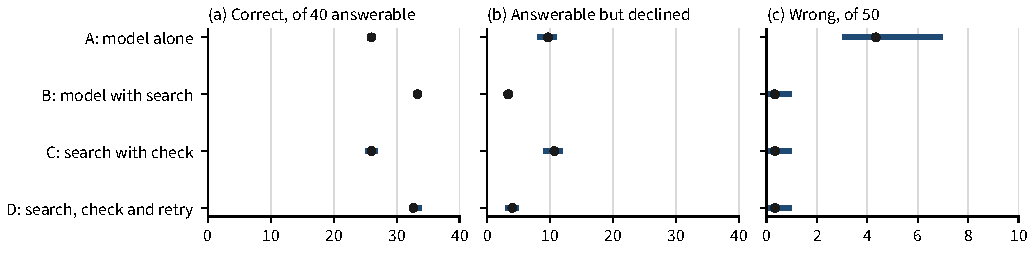
\includegraphics[width=\linewidth]{figures/results}
  \caption{Held-out results per arm. Each dot is the mean of three runs and the bar spans the lowest to the highest run. Panel (c) counts all 50 questions, since answering an unanswerable question is also wrong.}
  \label{fig:results}
\end{figure}

The model alone answered 26.0 of the 40 answerable questions correctly and gave a wrong answer to 4.3 questions per run, between 3 and 7. Its 13 wrong answers over three runs fell on seven questions. Two were wrong in every run, the BMA456 \texttt{INIT\_CTRL} reset value and the BMA456 sensor time increment discussed below, and two in two runs, the BMA456 filter bandwidth at an output data rate of \qty{100}{\hertz} and the BHI360 gyroscope sensitivity. Eight of the 13 answers said they came from memory or were uncertain; all 13 stated a value. One of the 13 answered an unanswerable question, and three are the sensor time answers, where the fault lies in the question; without those three, A gave 3.3 wrong answers per run.

With search, the model answered 33.3 correctly, refused all ten unanswerable questions in every run and gave one wrong answer in three runs. Every correct answer cited a page the question lists as stating the value. The three unplaced answers per run are correct when read by hand: each writes the unit against the number, as in \enquote{1.25ms}, \enquote{12.5MHz} and \enquote{0.4mm}, and the scorer's whole-word match does not find \enquote{ms} in \enquote{1.25ms}. The same three answers are unplaced in arms C and D.

The check alone withheld 22 of B's answers over the three runs, 7.3 per run, and every one was to an answerable question. Twelve quoted fewer than four words. Ten stated a number that no quote contained: in six the number was part of register notation, such as \enquote{bits 3..1} or \texttt{int\_latch='0'}, and in the rest an operating condition, a table number or a page number mentioned in passing. C's correct count fell to 26.0 and its false refusals rose from B's 3.3 to 10.7. The check removed none of B's wrong answers: the one wrong answer passed it.

With one revision, D revised all 22 withheld answers and showed 20, each scored correct. The two it still withheld were the same question in two runs: the answer repeated the field name \texttt{t\_sb[2:0]} from the question, and the check read 2 and 0 as numbers no quote contained. D answered 32.7 correctly with 4.0 false refusals: two answers in three runs behind B, 0.7 per run on each count.

The single wrong answer of arms B, C and D is the same answer in run 2 to the question of how often the BMA456 \texttt{SENSORTIME\_0} register increments. Page 16 of the datasheet says the register increments every \qty{39.25}{\micro\second}, and the question expects that value; pages 21 and 51 give \qty{39.0625}{\micro\second}~\cite{bma456}. In runs 1 and 3 the answer quoted both pages and stated both values, which the scorer accepts. In run 2 it quoted only pages 21 and 51 and gave \qty{39.0625}{\micro\second}, a value the datasheet does state. The model alone gave \qty{39.0625}{\micro\second} in all three runs. The datasheet contradicts itself, so these answers are scored wrong as committed but the fault lies in the question.

\Cref{tab:development} gives the development figures. They follow the same pattern with larger gaps: the check alone cost B 24.3 correct answers per run, and all 73 withheld answers passed the check after one revision, so a second revision was never requested. D's 0.3 shortfall against B is one revised answer, \enquote{1ms}, that is correct by hand but unplaced by the scorer. The limit was then lowered from two revisions to one, which leaves these figures unchanged and cuts the worst case from three requests per question to two.

\begin{table}[tbp]
  \centering
  \caption{Development set: 100 questions, 80 answerable, three runs per arm. These questions were read while the revision step was designed, so the figures show why it exists and are not the result. No arm returned an API error.}
  \label{tab:development}
  \begin{tabular}{
    l
    S[table-format=2.1] l
    S[table-format=2.1] l
    S[table-format=2.1] l
    S[table-format=2.1] l
    S[table-format=1.1] l
  }
    \toprule
    \head{Arm} & \multicolumn{2}{l}{\head{Correct}} & \multicolumn{2}{l}{\head{Wrong}} & \multicolumn{2}{l}{\head{Correct refusal}} & \multicolumn{2}{l}{\head{False refusal}} & \multicolumn{2}{l}{\head{Unplaced}} \\
    \midrule
    A: model alone & \runs{59.7}{58}{62} & \runs{11.0}{9}{13} & \runs{14.3}{13}{15} & \runs{15.0}{12}{17} & \steady{0.0} \\
    B: model with search & \steady{77.0} & \steady{0.0} & \steady{20.0} & \steady{3.0} & \steady{0.0} \\
    C: search with check & \runs{52.7}{52}{54} & \steady{0.0} & \steady{20.0} & \runs{27.3}{26}{28} & \steady{0.0} \\
    D: search, check and retry & \runs{76.7}{76}{77} & \steady{0.0} & \steady{20.0} & \steady{3.0} & \runs{0.3}{0}{1} \\
    \bottomrule
  \end{tabular}
\end{table}
